\documentclass[
	%a4paper, % Use A4 paper size
	letterpaper, % Use US letter paper size
]{jdf}

\addbibresource{references.bib}

\author{Andrew Myers}
\email{amyers72@gatech.edu}
\title{CS 7646: Project 8 - Brains vs. Bots: Trading with Instinct and Intelligence}

\begin{document}
%\lsstyle

\maketitle

\begin{abstract}
	Financial analysts have long been searching for ways to predict the future price of a stock.
	They have developed many "indicators" over time that are derived from historical data to help them make these predictions.
	Now, with the rise of machine learning, investors are more empowered then ever to make use of these indicators to create automated trading strategies.
	We will explore a Manual Strategy and a Machine Learning Strategy based off a Q-Learner to try and build profitable algorithms.
	We will compare the performance of these two strategies over historical data for JPM, and see how they perform in the presence of trading impact.
\end{abstract}

\section{Introduction}
Trading "Indicators" are data points derived from historical data for a stock that can be used to predict future price movements.
They are often used as inputs for trading strategies to determine when to buy or sell a stock. 
By using startegies that make decisions solely based on indicators, investors can automate their trading.
While this practice can create a trading bot, it takes a lot of human time to develop a strategy that is profitable.
However, with the advent of machine learning technologies, traders can now develop artifical intelligence algortihms to essentially design a strategy on its own.
In this report, we hypothesize that a machine learning "strategy learner" will perform better than a human-designed strategy.
To test this hypothesize, we will compare the performance of a human-designed strategy to a machine learning algorithm over historical pricing data for JPM in \textbf{Experiment 1}.
Then, we will look at the effect trading "impact" has on our strategy learner.
We hypothesize that a higher impact will cause our strategy portfolio to make less trades and result in a lower sharpe ratio for our portfolio.
We will test this by running our strategy learner with varying impact values in \textbf{Experiment 2}.

\section{Indicator Overview}
\subsection{Percentage Price Oscillator (PPO)}
Percentage Price Oscillator (PPO) is a momentum indicator that shows the relationship between the short-term and long-term moving averages of stock's price.
To calculate it, we first subtract the long-term moving average from the short-term moving average.
Then, we divide that value by the long-term moving average and multiply it by 100 to get a percentage.

We can tune the PPO by changing the short-term and long-term moving average periods.
In general, positive PPO values indicate that the short-term moving average is above the long-term moving average, which may indicate positive momentum.
For both the Manual Strategy and the Strategy Learner, we found that a short-term period of 5 days and a long-term period of 25 days worked well.
We used the thresholds of -2.0 and 2.0 to make buy and sell decisions in our Manual Strategy.

\subsection{Rate Of Change (ROC)}
Rate of Change (ROC) is also a momentum indicator.
This indicator shows how the price of a stock has changed over a certain period of time in order to identify trends.
We calculate ROC for a stock by taking the current closing price and subtracting the closing price from n days ago.
Then, we divide that value by the  n-day-old price price and multiply it by 100 to get a percentage.
If ROC is positive, it means the stock price has increased over the period, which could indicate positive momentum.
ROC may also indicate changes in trend directions when it crosses the zero line.
For both the Manual Strategy and the Strategy Learner, we found that a period of 30 days worked well.
We used the thresholds of -2.0 and 2.0 to make buy and sell decisions in our Manual Strategy.

\subsection{Fast Stochastic Oscillator (\%K)}
The Fast Stochastic Oscillator, or \%K, is a momentum indicator that compares a stock's closing price to it's high and low prices for each day over some time.
We calculate \%K by first finding the highest and lowest prices seen over the last n days.
Then, we subtract the lowest price seen from the current closing price, and divide that product by the difference between the highest and lowest prices.
Finally, we multiply that value by 100 to get a percentage.
The logic behind this indicator is that when a stock is overbought, it will be trading near its high price, and when it is oversold, it will be trading near its low price.
Therefore, a Fast Stochastic value of 80\% or higher is often used to signal that a stock is overbought, while a value of 20\% or lower is often used to signal that a stock is oversold.
For both the Manual Strategy and the Strategy Learner, we found that a period of 30 days worked well.
We used the thresholds of 20\% and 80\% to make buy and sell decisions in our Manual Strategy.

\section{Manual Strategy}
\subsection{Description}
We combined the indicators PPO, ROC, and \%K to create a manual strategy.
The logic of the strategy is to look for periods where both PPO and ROC agree on the trend of a stock price.
Then, we look for the \%K indicator to decide when to buy or sell, based on whether the stock is overbought or oversold.
We believe by relying on all three signals to agree before making any orders, we can effectively make profitiable trades.

In particular, we buy when:
\begin{itemize}
	\item BUY when PPO > -2.0 and ROC > -2.0 and \%K < 20\%
	\item SELL when PPO < 2.0 and ROC < 2.0 and \%K > 80\%
\end{itemize}

\subsection{Comparison and Evaluation}

\begin{jdffigure}
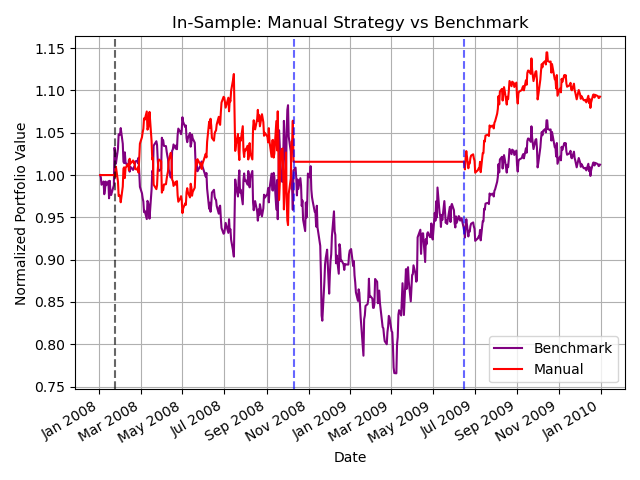
\includegraphics[height=6cm]{Project8Figures/Figure1.png}%
\captionof{figure}{Manual Strategy vs Benchmark Strategy during in-sample period of 2008-2009. Both portfolio values are normalized to 1. Blue vertical lines indicate LONG entrypoints, and Black lines indicate SHORT entrypoints.}\label{fig:figure}%
\end{jdffigure}
	
\textbf{Figure 1} shows the performance of our Manual Strategy when trading JPM during the in-sample period of Jan 1, 2008 to Dec 31, 2009.
We compare this strategy to a Benchmark Portfolio, which buys 1000 JPM shares on the first trading day and holds.
As we expected, our strategy outperforms the Benchmark Portfolio by a considerable margin.
There were only about 2 months over the 24 month period where the Benchmark Portfolio was more valuable.
One interesting thing to note is that the Manual Strategy value remained flat during the period where the Benchmark Strategy saw the largest dip.
Over this period, the Manual Strategy remained profitable by only holding cash. 
This was a winning strategy during the in-sample period.

Of course, it is expected that our Manual Strategy performs better during the in-sample period as that is the data we used to tune the strategy.
In particular, we tuned the lookback periods and thresholds until we found a strategy that is profitable for the in-sample period (exact values are available under \textbf{2. Indicator Overview}). 
However, we will next look at the performance of our strategy during the out-of-sample period of Jan 1, 2010 to Dec 31, 2011.

\begin{jdffigure}
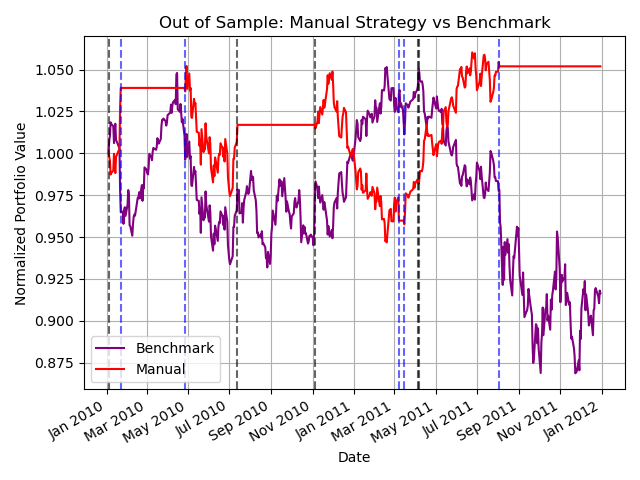
\includegraphics[height=6cm]{Project8Figures/Figure2.png}%
\captionof{figure}{Manual Strategy vs Benchmark Strategy during out-of-sample period of 2010-2011. Both portfolio values are normalized to 1. Blue vertical lines indicate LONG entrypoints, and Black lines indicate SHORT entrypoints.}\label{fig:figure}%
\end{jdffigure}

\textbf{Figure 2} shows that once again, the Manual Strategy outperforms the Benchmark Portfolio.
In fact, while the Benchmark Portfolio drops almost 10\% by the out-of-sample period, the Manual Strategy manages to walk away with an overall profit above 5\%.
However, the Manual Strategy did spend more months with a value below that of the Benchmark Portfolio.
In this case, it was about 6 months where the Benchmark Portfolio was worth more.
Once again though, we see that the Manual Strategy only held cash at times when the Benchmark Portfolio dropped to it's lowest value.

Looking at these results, it may be easy to assume that the Manual Strategy is a good strategy, as the out-of-sample results outperformed even the in-sample-results.
Again, this is not expected as we tuned the strategy to perform well on the in-sample data while being blind to out-of-sample data.
However, looking closely between both Figures 1 and 2, we see that the in-sample results look more consistent and stable than the out-of-sample results.
It seems like the in-sample-results would be profitable whenever the time period ended, whereas the out-of-sample results seemed to get lucky by being profitable right at the end of the period.
That being said, it is certainly promising that the Manual Strategy is also profitable during the out-of-sample period.


\section{Strategy Learner}
\subsection{High-Level Overview}
In order to see if we can build a better strategy than the Manual Strategy, we decided to use a Q-Learner.
The Q-Learner is a reinforcement learning algorithm that takes a discrete state space as input.
Based on these inputs, it is configured to return an action. 
In our case, the action can be one of 3 possible values: BUY, SELL, or HOLD.
A reward function is used to teach the Q-Learner which actions are best for which state.

To train our learner to make profitable trading decisions, we iterate through a period of historical dates and see what 'state' descrbed our indicators (PPO, ROC, and \%K) on that date. 
(Details about how to calculate state are below)
That 'state' is then submitted to the Q-Learner to get a suggested action.
We can calculate how profitable that action was by comparing to a price from a future date.
This profitability is used as our "reward".
This reward gets fed back into the Q-Learner and enables our algorithm to learn.
After running for some time, the Q-Learner will have learned to associate a "best" action for all of the possible states that it can encounter.

\subsection{Technical Details}
In order to train our Q-Learner, we first needed to descretize our inputs, PPO, ROC, and \%K.
For PPO, we assign a discrete value 0-4 based on which bin the indicator falls into on a given day:
\begin{itemize}
	\item < -2.0, -2.0 to -0.5, -0.5 to 0.5, 0.5 to 2.0, and > 2.0
\end{itemize}

For ROC, we also assign a value 0-4 based on 5 bins:
\begin{itemize}
	\item < -10.0, -10.0 to -2.0, -2.0 to 2.0, 2.0 to 10.0, and > 10.0
\end{itemize}

Lastly, for \%K, we assign a value 0-3 based on 4 bins:
\begin{itemize}
	\item 0 to 25.0, 25.0 to 50.0, 50.0 to 75.0, and 75.0 to 100.0
\end{itemize}

After finding the 3 correct buckets for a given day, we calculate a discrete state using the formula: \[state = (roc_bin * 20) + (ppo_bin * 4) + percentk_bin \]
There are 100 possible state combinations (5 * 5 * 4 = 100).

Next, we developed a reward function for the Q-Learner.
We calculated our reward by looking forward by 3 days to see if the action we took will be profitable or not.
This profit calculation takes into account the commission and impact of the trade. 
(Commission = 9.95 and Impact = 0.005, except in \textbf{Experiment 2}).
By rewarding the Q-Learner when we notice profitable trades, we hope it will learn to coninue that pattern in the future.
Similarly, unprofitable trades are penalized with a negative reward equal to the losses we project by looking forward 3 days.
Lastly, we set the reward function to penalize the Q-Learner with a reward of -30 when it decides to HOLD.
This is because we found that the boundaries already placed on our learners (Project 8 specifies the learner may only hold positions -1000, 0, and 1000 at a given time) made it difficult for the learner to make too many trades, even when there are many trade signals.
With these boundaries in place, we figured it best to incentivize our learner to send more BUY and SELL signals, rather than being more conservative and holding.

With a discretized state space and a reward function, we were finally able to train our model over in-sample data.
While training the Strategy Learner over the in-sample data, we manually tuned the parameters of the Q-Learner to find what produced the best results.
We found the best results with a learning rate (alpha) of 0.15, a discount factor (gamma) of 0.85, a random action rate (rar) of 0.5, and a random action decay (rard) of 0.999.
We did not find dyna hallucinations to be helpful.

We will compare the performance of our Q-Learner to the Manual Strategy in \textbf{Experiment 1} below.

\section{Experiment 1}
\subsection{Training Period}
In \textbf{Experiment 1}, we compare our Manual Strategy to our Strategy Learner over the in-sample period of Jan 1, 2008 to Dec 31, 2009.

\begin{jdffigure}
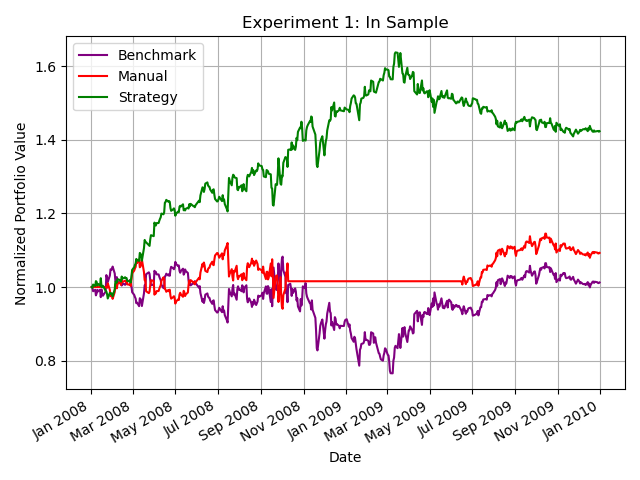
\includegraphics[height=6cm]{Project8Figures/Figure3.png}%
\captionof{figure}{Strategy Learner vs. Manual Strategy vs Benchmark Strategy during in-sample period of 2008-2009. Both portfolio values are normalized to 1.}\label{fig:figure}%
\end{jdffigure}

\textbf{Figure 3} shows the performance of our Manual Strategy and the Strategy Learner alongside our Benchmark Portfolio which holds 1000 shares.
As we hypothesized, the Strategy Learner outperforms the Manual Strategy by a signifcant margin with profit of ~42\% compared to ~10\%.
The Manual Strategy beats the Benchmark Portfolio, which sees hardly any profit.
While we are not suprised that the Strategy Learner beats the Manual Strategy which beats the Benchmark, it is interesting to see how well the Strategy Learner is able to perform.
It is worth noting, however, that the Strategy Learner is at high risk of overfitting it's model to the in-sample-data that it trained on.
Therefore, we should expect that the model does not perform as well when we look at out-of-sample data.

\subsection{Testing Period}
To see if the Strategy Learner can actually be profitable, we must test it against out-of-sample data as well. 
This out-of-sample data is from a period of time that was not used to help train the learner, and simulates potential "future" results.

\begin{jdffigure}
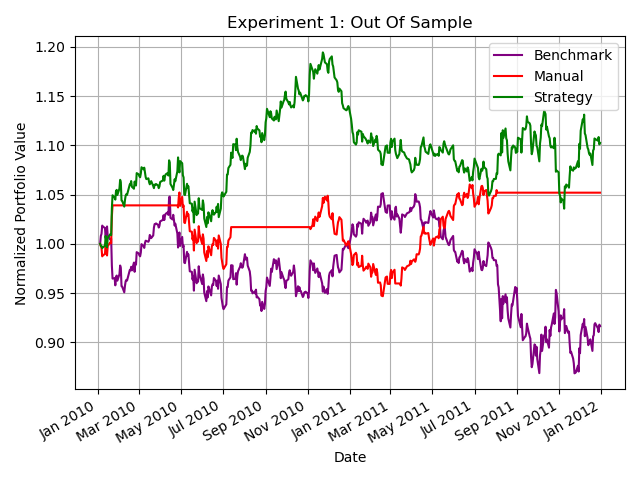
\includegraphics[height=6cm]{Project8Figures/Figure4.png}%
\captionof{figure}{Strategy Learner vs. Manual Strategy vs Benchmark Strategy during out-of-sample period of 2010-2011. Both portfolio values are normalized to 1.}\label{fig:figure}%
\end{jdffigure}

\textbf{Figure 4} shows that during the out-of-sample period, the Strategy Learner again performs best, followed by the Manual Strategy, and finally the Benchmark Portfolio.
In this case, the Strategy Learner only makes a profit of ~10\% over the 2 year period, while the Manual Strategy makes a profit of ~5\%.
Both of these strategies are winning for the investor, and especially beat out the Benchmark Portfolio which ends with an ~8\% loss.

In general, we'd expect that the Strategy Learner would perform best over most periods of data.
The Strategy Learner more adaptable to our indicators than we can be when tuning our Manual Strategy.
The Q-Learner can also learn over thousands of quick iterations instead of having an operator manually testing different paramters.
However, with the unpredictable nature of the stock marker, we are also sure that we can find time periods where our strategies don't perform as well.
In order to ensure a strategy can remain positive in the future, it would be valuable to test across many different time periods (this is an opportunity for future follow-up).

\section{Experiment 2}
In \textbf{Experiment 2}, we will consider how the trading impact of our orders influences the behavior of our Strategy Learner.
Impact is the price slippage that occurs during the execution of a buy or sell order.
If a trader buys a stock for \$100 with an impact of 0.05, the total cost would come out to \$100.05.
Inversely, a sale for \$100 with an impact of 0.05 would yield \$99.95.

We hypothesize that an increased impact will lead to fewer trades and a lower sharpe ratio for the portfolio.
This is because as impact goes up, the cost of trading increases.
This leads to higher costs that must be overcome to make profitable trades.
For this reason, we expect the Strategy Learner to make less trades overall when it has a higher impact.
The additional cost of trading also eats away slightly at profits, and slightly adds to the risk of each trade. 
For this reason, we expect the sharpe ratio to be lower when the impact is higher.
In this experiment, we test possible impact values of 0.001, 0.005, and 0.01.
Commission will be set to \$0 for this experiment.

\begin{jdffigure}
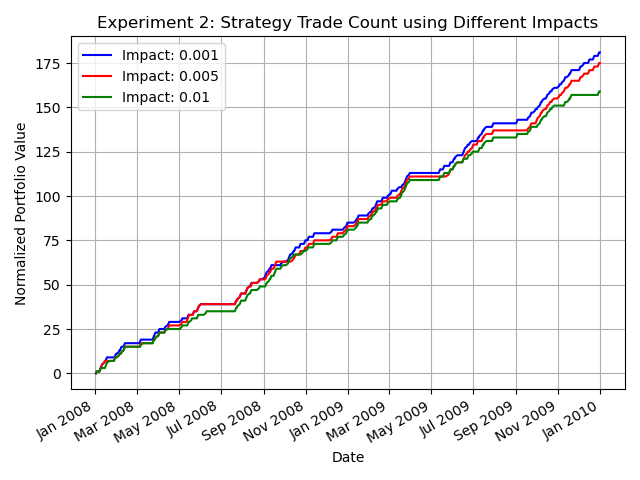
\includegraphics[height=6cm]{Project8Figures/Figure5.png}%
\captionof{figure}{Strategy Learner Trade Counts for Different Impact Values}\label{fig:figure}%
\end{jdffigure}

\textbf{Figure 5} shows the number of trades we made with the Strategy Learner over the in-sample period of 2008-2009.
As we expected, the Strategy Learner with an impact of 0.001had the most trades, followed by the Strategy Learner with an impact of 0.005, and finally the Strategy Learner with an impact of 0.01.

We can see the final count of trades alongside the sharpe ratios for each impact value in the table below.

\begin{jdffigure}
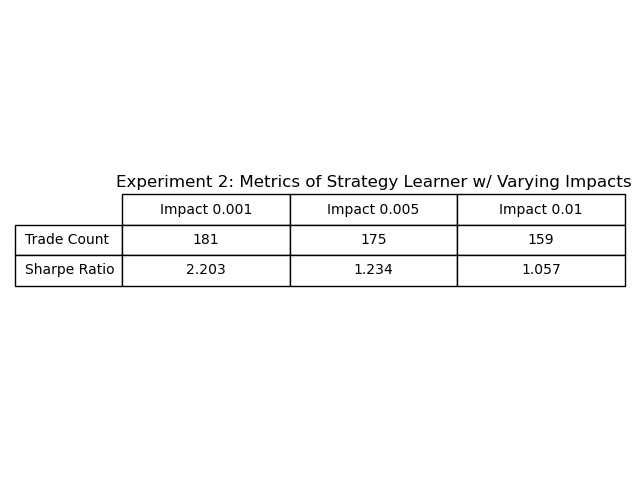
\includegraphics[height=6cm]{Project8Figures/Figure6.png}%
\captionof{figure}{Strategy Learner Final Trade Count and Sharpe Ratio for Different Impact Values}\label{fig:figure}%
\end{jdffigure}

As we can see in \textbf{Figure 1}, our hypotheses were correct.
The Strategy Learner with an impact of 0.001 made the most trades with 181 and had the highest sharpe ratio of 2.203.
The Strategy Learner with an impact of 0.005 made 175 trades and had a sharpe ratio of 1.234.
Finally, the Strategy Learner with an impact of 0.01 made only 159 trades and had a sharpe ratio of 1.057.
This supports our hypothesis that higher impact leads to fewer trades and a lower sharpe ratio, due to the higher costs of the trades.


\end{document}
